% Proposed-methods manuscript. No new foundation-model experiment is reported.
% Build from this directory: tectonic --keep-logs --keep-intermediates main.tex
\documentclass[conference]{IEEEtran}
\usepackage[T1]{fontenc}
\usepackage{cite}
\usepackage{amsmath,amssymb}
\usepackage{graphicx,booktabs,array}
\usepackage{xurl}
\usepackage[hidelinks]{hyperref}
\hypersetup{pdftitle={Frozen Encoders for Few-Shot Rare Retinal OCT Classification: A Proposed Evaluation Protocol},pdfauthor={Doan Tung Lam, Ha Quang Minh, Pham Duc Anh, Ngo Hoang Phuc}}
\newcommand{\R}{\mathbb{R}}
\newcommand{\Kdev}{\mathcal{K}_{\mathrm{dev}}}
\newcommand{\rare}{\mathcal{C}_{\mathrm{rare}}}
\newcommand{\claim}[1]{} % Stable identifiers join prose to CLAIM_SOURCE_LEDGER.md.
% IEEEtran.bst's documented control-entry citation avoids a printed reference.
\makeatletter
\def\bstctlcite{\@ifnextchar[{\@bstctlcite}{\@bstctlcite[@auxout]}}
\def\@bstctlcite[#1]#2{\@bsphack
  \@for\@citeb:=#2\do{%
    \edef\@citeb{\expandafter\@firstofone\@citeb}%
    \if@filesw\immediate\write\csname #1\endcsname{\string\citation{\@citeb}}\fi}%
  \@esphack}
\makeatother
\begin{document}
\bstctlcite{IEEEcontrol}
\title{Frozen Encoders for Few-Shot Rare Retinal OCT\linebreak Classification: A Proposed Evaluation Protocol}
\author{\IEEEauthorblockN{Doan Tung Lam, Ha Quang Minh, Pham Duc Anh, Ngo Hoang Phuc}
\IEEEauthorblockA{National Economics University}}
\maketitle

\begin{abstract}
Rare retinal disease recognition from optical coherence tomography (OCT) is constrained by scarce labels and uncertain transfer across sources. This paper proposes a comparison of frozen foundation models (FMs)---RETFound Nature OCT, DINOv2-Base and MIRAGE-Base---with a matched Keras Inception-v3 reference. Five-way classification will use identical real-image supports, primary cosine prototypes and a secondary fixed-regularization logistic probe. Five grouped development folds and paired nested support draws will guide a prespecified nomination; legacy and external outcomes will not revise that choice. A separate nine-way audit will measure false rare predictions on NORMAL images from Kermany, OCTID and OCTDL, subject to access and eligibility checks. The protocol distinguishes support budgets from all inspected development labels, screens dependence and preserves historical artifacts. No new FM results are reported. The contribution is an auditable, descriptive evaluation with explicit limits on patient independence, pretraining exposure and clinical interpretation.
\end{abstract}
\begin{IEEEkeywords}
optical coherence tomography, rare retinal disease, few-shot learning, frozen encoders, source shift
\end{IEEEkeywords}

\section{Introduction and Problem Statement}
\claim{C01}
Optical coherence tomography (OCT) provides cross-sectional retinal images for disease classification. Transfer learning has supported recognition of common OCT categories, as illustrated by Kermany et al.\ \cite{Kermany2018}, whereas Yoo et al.\ \cite{Yoo2021} studied the more restricted image supply of five rare diseases. For this collection, the practical question is whether pretrained representations can distinguish those five diseases from a small number of labelled supports, and whether a classifier that also recognizes common conditions mistakes a new source of normal scans for rare pathology. These are related but distinct questions.

\claim{C02}
The historical reproduction used four common categories---NORMAL, choroidal neovascularization (CNV), diabetic macular edema (DME) and DRUSEN---and five rare categories. Frozen Inception-v3 features fed a softmax head trained with real-only, basic-augmentation or CycleGAN-augmentation pools. Table~\ref{tab:history} reports archived outputs, not directly comparable K-shot results. The ordering changed between seed 42 and the five-seed descriptive means, motivating paired evaluation without establishing GAN superiority or equivalence to basic augmentation.

\begin{table}[t]
\caption{Historical project accuracy (\%); nine-way, fixed legacy test. No new FM scores.}
\label{tab:history}
\centering
\begin{tabular}{lrr}
\toprule
Rare training pool & Seed 42 & Seeds 1--5, mean $\pm$ SD\\
\midrule
Real only & 90.31 & $90.69\pm1.86$\\
Basic augmentation & 88.85 & $92.93\pm1.85$\\
CycleGAN augmentation & 92.95 & $92.59\pm1.29$\\
\bottomrule
\end{tabular}
\par\smallskip
\parbox{\columnwidth}{\footnotesize Sources: archived \texttt{results/stage4/metrics.csv} and \texttt{results/seed\_check.csv}; SD across the five listed training seeds. The same test images were reused.}
\end{table}

\claim{C03}
Validity concerns also motivate the new design. The project's prior format/framing audit retained strong rare-versus-common feature separation (area under the curve approximately 0.995 before and 0.991 after framing normalization). Disease and dataset source were confounded, so this diagnostic did not identify a mechanism. The fixed Kermany test also contains patients present in the fitting split.\footnote{Archived evidence: \texttt{results/c0/v1\_gate\_summary.csv} and \texttt{docs/research/CONTEXT.md}; exact quantities and provenance are mapped in the accompanying claim ledger.} Grouping cannot repair that overlap while preserving this legacy benchmark. A five-way rare-only task removes the common-versus-rare output decision, while a separate source audit asks whether normal scans are assigned rare labels; neither guarantees removal of within-rare acquisition cues.

\claim{C04}
The contribution is a fixed-checkpoint comparison under matched support-label budgets with a source-dependent error audit, not a new encoder, adaptation algorithm or first rare-eye foundation-model application. Finalized protocol v1.0 (5 November 2026) and a claim ledger accompany this draft. All new extraction, grouping, selection and inference below remain proposed.

\section{Related Work}
\subsection{Rare Retinal Recognition and Pretrained Representations}
\claim{C05}
Yoo et al.\ \cite{Yoo2021} augmented rare OCT classes with per-disease CycleGAN translation before nine-way classification. Quellec et al.\ \cite{Quellec2020} detected rare fundus pathologies using representations learned for frequent conditions. These establish rare-retinal few-shot precedents, but fundus differs from OCT, and inventory-wide augmentation differs from fitting on only $K$ real supports per class.

\claim{C06}
RETFound learns representations from retinal images and evaluates downstream disease detection with label-efficiency analyses \cite{RETFound2023}. MIRAGE combines OCT and scanning-laser ophthalmoscopy pretraining and benchmarks multiple OCT tasks \cite{MIRAGE2025}. EyeCLIP adds multimodal visual-language learning and few-shot/zero-shot ophthalmic evaluations \cite{EyeCLIP2025}. DINOv2 supplies a general visual self-supervised comparator \cite{DINOv2}; generalist-versus-specialist ocular comparisons already exist \cite{Generalist2025}. These studies motivate the selected checkpoints, but their adaptation procedures, cohorts and model capacities do not predict a winner for the present frozen-cosine task. RETFound's documented Kermany-related pretraining exposure also prevents treating the matched legacy reference as an upstream-exposure-controlled experiment.

\claim{C07}
EyeDiff already combines synthetic ophthalmic images and foundation models for rare-disease tasks \cite{EyeDiff2026}, precluding that novelty claim here. The project's generators and automatic feature-distance quality control used the broader rare training inventory; subsampling outputs cannot undo that exposure. Synthetics are excluded from this strict K-shot comparison. Visual plausibility and diagnostic utility are separate endpoints.

\subsection{Lessons from Few-Shot Learning Across Fields}
\claim{C08}
Prototypical Networks learn an embedding in which class prototypes support few-shot recognition \cite{ProtoNets2017}. SimpleShot shows the importance of simple feature transformations and nearest-neighbor baselines \cite{SimpleShot2019}. The present classifier instead uses already pretrained, frozen encoders and explicitly normalized cosine centroids; it is neither a newly trained Prototypical Network nor an exact SimpleShot implementation. Cross-domain evaluation spanning satellite, dermatology and X-ray imagery \cite{CrossDomain2020} further cautions against importing rankings from natural-image benchmarks into OCT.

\claim{C09}
Resource accounting is equally important. STARTUP adapts representations with unlabelled target-domain images \cite{STARTUP2021}; that access is additional information excluded here. In natural language processing, Mosbach et al.\ \cite{FairNLP2023} show why adaptation comparisons must control model and example budgets. CLAP's analysis of vision-language adaptation highlights target-specific tuning and distribution-shift sensitivity \cite{CLAP2024}; its text-initialized, constrained probe is not the fixed-L2 logistic probe specified below. These lessons support matched episodes and explicit development-label disclosure, not a universal claim that linear probes win.

\claim{C10}
Prompt methods also change the computational and supervision contract. CoCoOp conditions learned text prompts on input images \cite{CoCoOp2022}; PathPT combines textual prompt tuning with spatial aggregation and tile supervision for rare-cancer pathology \cite{PathPT2026}. Neither is a drop-in image-only OCT comparator or evidence that a small trainable parameter count guarantees low total cost. Retinal shift evaluation itself has precedents, including BenchReAD's cross-dataset anomaly-detection benchmark \cite{BenchReAD2025}. Anomaly detection, however, differs from naming five diseases or counting NORMAL scans assigned any rare label. This study isolates frozen adaptation and measures its own costs rather than extending the sprint to prompts, adapters or full fine-tuning.

\section{Proposed Methods}
\begin{figure*}[t]
\centering
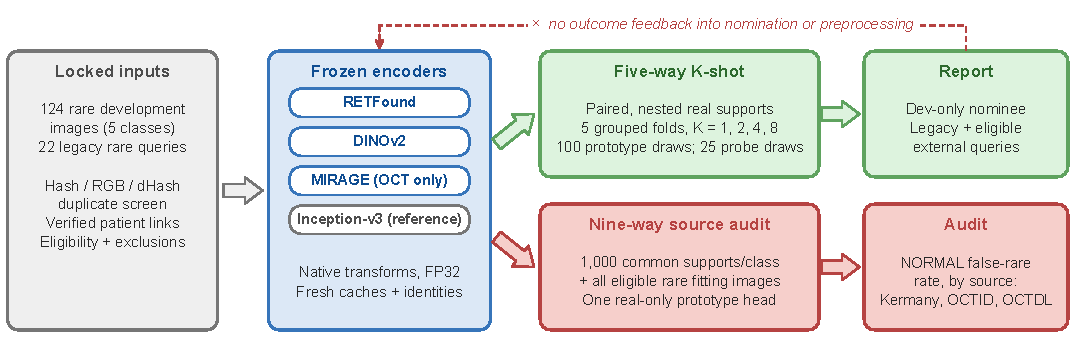
\includegraphics[width=\textwidth]{methods_figure.pdf}
\caption{Proposed protocol; all boxes denote planned operations. Shared locked image identities and frozen checkpoint pipelines feed two distinct analyses. The five-way branch uses paired K-shot supports and development-only nomination. The nine-way branch uses a separate, deterministic real-only fitting roster to measure false-rare rate (FRR) on NORMAL scans. External inventories and final query IDs are locked before their inference. Image-similarity groups do not establish patient identity. No outcome from either reporting branch feeds back into nomination or preprocessing.}
\label{fig:methods}
\end{figure*}

\subsection{Tasks, Data and Information Budgets}
\claim{C11}
The primary task is closed-set classification of central serous chorioretinopathy (CSC), macular hole (MH), macular telangiectasia (MacTel), Stargardt disease and retinitis pigmentosa (RP). In that fixed order, the canonical manifest contains $27/26/25/19/27$ real development images (124 total) and $5/5/4/4/4$ legacy queries (22 total). There are no real rare validation rows. The full manifest has 84,630 images: 74,082 training, 9,526 validation and 1,022 test. It will remain unchanged; derived rosters reference its paths. Counts describe images, not verified independent patients.

\claim{C12}
A five-way $K$-shot head uses $5K$ labelled supports. The separate, unique inspected development-label budget is 124: supports are drawn from that inventory, not added to it or multiplied by folds and draws. The 22 rare evaluation labels have been historically inspected, so the legacy query set is not newly blind. Common fitting labels and upstream pretraining exposure will be disclosed separately. No synthetic supports, stochastic augmentation, unlabelled-target self-training, query adaptation, fitted feature scaler or query-updated normalization will be used.

\subsection{Dependence Screening and Feasibility Gates}
\claim{C13}
Before new-protocol scores, the 146 rare benchmark images will be screened using equal file hashes and equal decoded RGB pixels with dimensions. Alpha is discarded only for the RGB fingerprint; original hashes are retained. A fixed 64-bit horizontal difference hash will flag pairs at Hamming distance $\leq4$: Pillow RGB-to-L conversion, BOX resize to $9\times8$, row-major adjacent left-greater-than-right bits. Decoder/Pillow versions will be pinned. This is a candidate screen, not a validated patient detector. Raw-image review without new encoder scores will place confirmed or unresolved possible duplicates in connected components. Conflicting image labels block the affected component pending resolution.

\claim{C14}
Rare fitting components linked to legacy queries will be excluded before fitting lock; canonical test rows will not move. Development groups will union image components with verified, dataset-namespaced patient links where available. Unknown patients remain unknown. A verified rare patient spanning disease labels stops the selector for a prescore fold amendment. Group IDs are minimum normalized POSIX member paths; class-specific inventories are sorted case-sensitively. A fixed PCG64 permutation followed by round-robin assignment gives five folds. Every fold must contain all five query classes and eight fitting groups per class, requiring at least ten eligible groups per class. Any failure stops the entire selector before scores; no favorable fold omission or automatic reduction of $K$ is allowed.

\subsection{Frozen Checkpoint Pipelines and Feature Identity}
\claim{C15}
The fixed roster is RETFound Nature OCT, DINOv2-Base and MIRAGE-Base (OCT-only inference), with an ImageNet Keras Inception-v3 reference (Table~\ref{tab:roster}). BioMedCLIP image features replace RETFound only for predefined access, loading or terms failure, before new labelled comparisons. Failure of another arm or the fallback reduces the roster without a checkpoint search; unavailable arms are not scored as poor models. An arm unavailable at input lock cannot enter nomination later in v1.

\begin{table}[t]
\caption{Fixed checkpoint identities; exact revisions and transforms await the prescore gate.}
\label{tab:roster}
\centering\footnotesize
\begin{tabular}{@{}p{0.22\columnwidth}p{0.70\columnwidth}@{}}
\toprule
Arm & Public identity / reference implementation\\
\midrule
RETFound & \path{YukunZhou/RETFound_mae_natureOCT}\\
DINOv2 & \path{facebook/dinov2-base}\\
MIRAGE & \path{j-morano/MIRAGE-Base}, OCT only\\
Conditional fallback & \path{microsoft/BiomedCLIP-PubMedBERT_256-vit_base_patch16_224}, image only\\
Inception-v3 & Historical Keras ImageNet loading/backbone; $256\to299$ resize and global average pooling\\
\bottomrule
\end{tabular}
\end{table}

\claim{C16}
The gate will pin usable terms, weight revision/hash, channel handling, deterministic native transforms, normalization, pooling, dtype and inference mode. Checkpoint-native preprocessing will be retained, with crop geometry and retained field-of-view fraction logged by image/source. Fresh matched features, including the Keras reference, will use FP32 inference and raw float32 storage; CPU normalization and classifier arithmetic will use float64. Cache identity will include ordered image IDs/content hashes, weights, transforms/pooling, environment, dimension/dtype and code revision. Historical float16 Inception caches cannot recover the original precision and lack this identity contract; they and saved nine-way heads remain historical artifacts. Nonfinite or zero-norm features/centroids stop the arm.

\subsection{Primary Prototypes and Secondary Logistic Probes}
\claim{C17}
Let $f_m(x)\in\R^{d_m}$ be encoder $m$'s embedding, and $S_c$ contain the $K$ supports for class $c$. The primary head will compute
\begin{align}
u_m(x)&=\frac{f_m(x)}{\|f_m(x)\|_2},\quad
a_{m,c}=\frac{1}{K}\sum_{x\in S_c}u_m(x),\\
p_{m,c}&=\frac{a_{m,c}}{\|a_{m,c}\|_2},\quad
\widehat y(x)=\arg\max_c u_m(x)^\top p_{m,c}.
\label{eq:proto}
\end{align}
Exact ties follow CSC/MH/MacTel/Stargardt/RP order. Normalizing every support before averaging is essential: the historical raw-feature Euclidean prototype and raw-mean cosine helper do not implement this rule. No post-hoc centering will be added to improve an observed model ranking.

\claim{C18}
The secondary five-way probe will use the same unit features and balanced supports, minimizing
\begin{equation}
\begin{aligned}
\mathcal{L}(W,b)={}&-\frac{1}{5K}\sum_{(x,y)\in S}
\log\!\left[\operatorname{softmax}(Wu_m(x)+b)\right]_y\\
&+0.005\|W\|_F^2.
\end{aligned}
\label{eq:logistic}
\end{equation}
The intercept is unpenalized; initialization is zero, with no imbalance weights. Analytic gradients and L-BFGS-B will use \texttt{maxiter=1000}, \texttt{maxfun=20000}, \texttt{maxls=20}, \texttt{maxcor=10}, \texttt{gtol=1e-6} and \texttt{ftol=0}, without bounds. Convergence requires finite parameters/objective and maximum absolute gradient $\leq10^{-6}$; actual termination reasons and missing pairs will be reported. A fixed library $C$ or the historical Adam head is not a substitute for this mean-loss objective. No regularization or draws will be replaced after viewing query outcomes.

\subsection{Paired Episodes, Nomination and Reporting}
\claim{C19}
Development will evaluate $\Kdev=\{1,2,4,8\}$ with 100 nested support draws per fold. Each draw permutes fitting groups, selects one uniformly chosen image per group, and uses prefixes for increasing $K$. Every encoder/classifier shares those IDs and within-group choices; fold queries contain all eligible held-out rows. Reporting will instead draw from all eligible development groups and evaluate $K\in\{1,2,4,8,16\}$ on the legacy queries and eligible external subsets. If any class has fewer than 16 fitting groups, $K=16$ will be omitted for every encoder. The secondary probe uses development $K=4$, first 25 matching draws per fold, and the first 25 matching reporting draws per $K$. Exact PCG64/SeedSequence namespaces and path-order rules are archived in protocol sections 4 and 6; realized support/query IDs will be saved, not seeds alone.

\claim{C20}
Primary performance is macro recall; ordinary accuracy, class recalls and confusion counts are secondary. Nomination uses complete prototype development results only. For model $m$, with $q_{f,c}$ held-out class counts and $h_{m,K,r,f,c}$ correct predictions,
\begin{equation}
S_m=\frac{1}{4\cdot100}\sum_{K\in\Kdev}\sum_{r=1}^{100}
\frac{1}{5}\sum_{c\in\rare}\frac{\sum_{f=1}^{5}h_{m,K,r,f,c}}{\sum_{f=1}^{5}q_{f,c}}.
\label{eq:nomination}
\end{equation}
Pooling correctness within each class before averaging avoids equally weighting unequal fold class counts. Only FMs completing every required fold/$K$/draw can enter nomination; at least two complete FMs are required. Inception is a reference, not a candidate winner. Partial averages remain descriptive and cannot select a primary model.

\claim{C21}
Among complete FMs within 0.02 of the best $S_m$, the nominee will have the lowest median warm extraction seconds/image. Timing uses the same fixed, prescore-ordered 100-image development inventory, repeating IDs only for timing if needed, batch one, FP32, one warm pass and five timed passes on the same hardware/session. Each statistic is the median of the five per-pass mean times; preprocessing is included, download/disk I/O excluded, with GPU synchronization. Models run sequentially in RETFound/DINOv2/MIRAGE order, one process each; hardware changes require retiming all candidates. Final ties use that order, with BioMedCLIP occupying RETFound's slot. This two-percentage-point rule allocates engineering effort; it is not equivalence. The primary nominee will be locked before legacy/external outcomes, and every model will remain reported. Without valid nomination, all reporting is exploratory.

\claim{C22}
Reporting will show paired nominee-minus-Inception macro-recall differences by $K$, plus all secondary model contrasts, using shared completed episodes and available/planned counts. Support-draw mean, SD and fifth/ninety-fifth percentiles describe example-selection variability conditional on these images. They are not patient confidence intervals; repeated draws create no new patients. No confirmatory $p$-values, episode standard errors or automatic superiority/equivalence claims are planned. Selection also makes the nominee's development estimate optimistic.

\subsection{Separate Nine-Way Source Audit}
\claim{C23}
Each encoder will receive exactly one deterministic real-only nine-way prototype head using (1)--(2), with the average taken over all selected supports. The common fitting roster is the identical seed-42 sample of 1,000 images per common class, selected with \texttt{major\_indices} from the full 73,958-row common fitting frame and mapped back to paths in order. All eligible real rare fitting images are appended. Common rows will not be removed by the rare exclusion rule. Before exclusions and external additions, the shared extraction inventory is $4{,}000+1{,}000+146=5{,}146$ images per encoder. No common-validation extraction, optimizer seeds or synthetic images enter this audit.

\claim{C24}
Class order is fixed: NORMAL, CNV, DME, DRUSEN, CSC, MH, MacTel, Stargardt and RP. For each source $s$, false-rare rate is
\begin{equation}
\operatorname{FRR}_s=
\frac{\#\{x\in N_s:\widehat y(x)\in\rare\}}{|N_s|},
\end{equation}
where $N_s$ contains eligible true NORMAL queries. Kermany, OCTID \cite{OCTID2020} and OCTDL \cite{OCTDL2024} will be reported separately, alongside NORMAL recall, common confusions, rare recall and all denominators. Low FRR alone is insufficient if rare disease recognition is poor. A five-way rare-only head has no NORMAL output and cannot supply this diagnostic.

\claim{C25}
External release/hash, terms, label inventory and eligibility rules will be frozen before outcomes. External queries will be screened against every locked fitting row, legacy queries and one another using the same image screen and verified patient links. Fitting/legacy-linked external components will be excluded without changing locked fitting rosters; within-query dependence remains recorded. Final external query IDs will be frozen before inference. Screening coverage will be stated: unused legacy images and private pretraining overlap remain unknown. Rare transfer is conditional on verified labels, including clinical CSR-to-CSC equivalence. OCTDL's broad condition labels do not automatically identify MH. Partial-class cohorts will retain all five output classes and report present-class recalls/output allocations, not a five-class macro recall. All nine output allocations will remain visible in the source audit. Cosine scores will not be labelled probabilities; logistic outputs will include probabilities in fixed order.

\claim{C26}
For deterministic nine-way outputs, optional descriptive 95\% percentile intervals will use 5,000 patient-cluster draws (seed zero) only where verified IDs exist. Otherwise, image/duplicate-group conditional intervals will be explicitly labelled. Intervals condition on the fitted head and omit development-selection uncertainty. Common-patient overlap remains a legacy limitation rather than being repaired by clustering.

\section{Discussion and Execution Boundaries}
\claim{C27}
Joint rare recognition and NORMAL source auditing address a practical ambiguity: accurate rare discrimination may coexist with false rare predictions on a new source, while low FRR may coexist with weak rare recall. These outcomes cannot isolate morphology, acquisition, preprocessing, capacity or pretraining effects. Five-way restriction and duplicate screening address specific dependencies without establishing patient independence or clinical transportability.

\claim{C28}
With four or five legacy queries per rare class, one prediction moves recall by 0.25 or 0.20. Historically inspected labels, unknown rare patients, upstream exposure and incomplete external disease coverage limit population claims. Larger $K$ creates overlapping support rosters; narrow draw spread need not mean population precision. Documented failures and infeasible arms will remain part of the evidence.

\claim{C29}
An isolated Colab PyTorch extractor/evaluator, with Keras for Inception and CPU classifiers, will use one Colab Pro GPU session at a time. Generation, augmentation sweeps, prompts, adapters and backbone fine-tuning are excluded. Runtime, peak RAM/VRAM and download, staging, extraction, fitting and serialization costs will be recorded separately; GPU-hour savings remain unmeasured. New versioned outputs will preserve canonical data, heads and historical results.

\claim{C30}
Before labelled comparisons, a local input lock will archive protocol, roster, grouping, episode, checkpoint, transform, code/environment and endpoint identities. This is not public preregistration. Predictions, counts, failures and completion hashes will support identity-checked resumption. Failed external NORMAL access yields a rare-only pilot; failed rare mapping removes that transfer claim. Numerical/identity failure stops the arm; required-fold failure stops selection. Dated amendments preserve previous outputs.

\claim{C31}
The 11 November submission reports proposed methods without new FM outcomes. Planned November milestones are implementation/input checks (12--14), paired development/nomination (15--19), locked query reporting (20--23) and evidence freeze (27). Access, loading, grouping and clinical mappings remain unpassed gates. Late delivery will drop secondary probes first and disclose reduced scope, without waiting for favorable outcomes.

\section{Conclusion}
Shared episodes, explicit label accounting and development-only nomination make the proposed frozen-encoder comparison inspectable. The companion nine-way audit addresses source-dependent errors. Historical augmentation findings motivate, but do not answer, these questions. Outcomes and feasibility will be reported without causal pretraining, patient-independent validation or clinical-benefit claims beyond the evidence.

\section*{Writing and Reproducibility Note}
The authors remain responsible for this work. Codex assisted drafting, figures and source checking with research skills \cite{Kassis2026}, acknowledged as tooling only. The source ledger and protocol accompany this draft for author review.

\bibliographystyle{IEEEtran}
\bibliography{references}
\end{document}
